%!TEX root = handout.tex

\newpage
\section{OpenSWATH}
\subsection{Introduction}

OpenSWATH~\cite{Rost2014fd} is a module of OpenMS that allows analysis of LC-MS/MS DIA (data independent acquisition) data using the approach described by Gillet \textit{et~al.}~\cite{Gillet2012Targeted}. The DIA approach described there uses 32 cycles to iterate through precursor ion windows from 400-426 Da to 1175-1201 Da and at each step acquires a complete, multiplexed fragment ion spectrum of all precursors present in that window. After 32 fragmentations (or 3.2 seconds), the cycle is restarted and the first window (400-426 Da) is fragmented again, thus delivering complete ``snapshots'' of all fragments of a specific window every 3.2 seconds.

The analysis approach described by Gillet et al. extracts ion traces of specific fragment ions from all MS2 spectra that have the same precursor isolation window, thus generating data that is very similar to SRM traces.

\subsection{Installation of OpenSWATH}
OpenSWATH has been fully integrated since OpenMS 1.10 (\url{http://open-ms.sourceforge.net} \cite{Kohlbacher2007,Sturm2008,Bertsch2011OpenMS}).

\subsection{Installation of mProphet}
mProphet (\url{http://www.mprophet.org/}) \cite{Reiter2011MProphet} is available as standalone script in \directory{External\_Tools/mProphet/}. 
R (\url{http://www.r-project.org/}) and the package MASS (\url{http://cran.r-project.org/web/packages/MASS/}) are further required to execute mProphet. 
Please obtain a version for either Windows, Mac or Linux directly from CRAN.

pyprophet, a much faster reimplementation of the mProphet algorithm is available from PyPI (\url{https://pypi.python.org/pypi/pyprophet/}). The usage of pyprophet instead of mProphet is suggested for large-scale applications, but the installation requires more dependencies and therefore, for this tutorial the application of mProphet is described.

\subsection{Generating the Assay Library}
\subsubsection{Generating TraML from transition lists}
OpenSWATH requires the assay libraries to be supplied in the TraML format \cite{Deutsch2012TraMLA}. To enable manual editing of transition lists, the TOPP tool \OPENMSTOOL{ConvertTSVToTraML} is available that uses tab separated files as input. Example datasets are provided in \directory{OpenSWATH/assay/}. Please note that the transition lists need to be named \texttt{.csv} or \texttt{.tsv}.

The header of the transition list contains the following variables (with example values in brackets):

\begin{description}
  \item[\texttt{PrecursorMz}] \hfill \\
  The mass-to-charge (m/z) of the precursor ion. (728.88)
  \item[\texttt{ProductMz}] \hfill \\
  The mass-to-charge (m/z) of the product or fragment ion. (924.539)
  \item[\texttt{Tr\_recalibrated}] \hfill \\
  The \textbf{normalized} retention time (or iRT) \cite{Escher2012Using} of the peptide. (26.5)
  \item[\texttt{transition\_name}] \hfill \\
  A \textbf{unique} identifier for the transition.\\
  (AQUA4SWATH\_HMLangeA\_ADSTGTLVITDPTR(UniMod:267)/2\_y8)
  \item[\texttt{CE}] \hfill \\
  The collision energy that should be used for the acquisition. (27)\\
  \texttt{Optional} (not used by OpenSWATH)
  \item[\texttt{LibraryIntensity}] \hfill \\
  The relative intensity of the transition. (3305.3)
  \item[\texttt{transition\_group\_id}] \hfill \\
  A \textbf{unique} identifier for the transition group.\\
  (AQUA4SWATH\_HMLangeA\_ADSTGTLVITDPTR(UniMod:267)/2)
  \item[\texttt{decoy}] \hfill \\
  A binary value whether the transition is target or decoy (target:0, decoy:1). (0)
  \item[\texttt{PeptideSequence}] \hfill \\
  The unmodified peptide sequence. (ADSTGTLVITDPTR)
  \item[\texttt{ProteinName}] \hfill \\
  A unique identifier for the protein. (AQUA4SWATH\_HMLangeA)
  \item[\texttt{Annotation}] \hfill \\
  The fragment ion annotation. (y8)\\
  \texttt{Optional} (not used by OpenSWATH)
  \item[\texttt{FullUniModPeptideName}] \hfill \\
  The peptide sequence with UniMod modifications. (ADSTGTLVITDPTR(UniMod:267))
  \item[\texttt{MissedCleavages}] \hfill \\
  The number of missed cleavages during enzymatic digestion. (0)\\
  \texttt{Optional} (not used by OpenSWATH)
  \item[\texttt{Replicates}] \hfill \\
  The number of replicates. (0)\\
  \texttt{Optional} (not used by OpenSWATH)
  \item[\texttt{NrModifications}] \hfill \\
  The number of modifications. (0)\\
  \texttt{Optional} (not used by OpenSWATH)
  \item[\texttt{PrecursorCharge}] \hfill \\
  The precursor ion charge. (2)
  \item[\texttt{GroupLabel}] \hfill \\
  The stable isotope label. (light)\\
  \texttt{Optional} (not used by OpenSWATH)
  \item[\texttt{UniprotID}] \hfill \\
  The Uniprot ID of the protein. ()\\
  \texttt{Optional} (not used by OpenSWATH)
\end{description}

To convert transitions lists to TraML, use \OPENMSTOOL{ConvertTSVToTraML}:\\

\begin{description}
  \item[Linux or Mac] \hfill \\
    On the Terminal:
    \begin{lstlisting}
  ConvertTSVToTraML -in OpenSWATH_SGS_AssayLibrary.csv -out OpenSWATH_SGS_AssayLibrary.TraML
  \end{lstlisting}
  \item[Windows] \hfill \\
    On the TOPP command line:
    \begin{lstlisting}
  ConvertTSVToTraML.exe -in OpenSWATH_SGS_AssayLibrary.csv -out OpenSWATH_SGS_AssayLibrary.TraML
  \end{lstlisting}
\end{description}

\subsubsection{Appending decoys to a TraML}
In addition to the target assays, OpenSWATH further requires decoy assays in the library which are later used for classification and error rate estimation. For the decoy generation it is crucial that the decoys represent the targets in a realistic but unnatural manner without interfering with the targets. The methods for decoy generation implemented in OpenSWATH include 'shuffle', 'pseudo-reverse', 'reverse' and 'shift'. To append decoys to a TraML, the TOPP tool \OPENMSTOOL{OpenSwathDecoyGenerator} can be used:

\begin{description}
  \item[Linux or Mac] \hfill \\
    On the Terminal:
    \begin{lstlisting}
  OpenSwathDecoyGenerator -in OpenSWATH_SGS_AssayLibrary.TraML -out OpenSWATH_SGS_AssayLibrary_with_Decoys.TraML -method shuffle -append -exclude_similar -remove_unannotated
  \end{lstlisting}
  \item[Windows] \hfill \\
    On the TOPP command line:
    \begin{lstlisting}
  OpenSwathDecoyGenerator.exe -in OpenSWATH_SGS_AssayLibrary.TraML -out OpenSWATH_SGS_AssayLibrary_with_Decoys.TraML -method shuffle -append -exclude_similar -remove_unannotated
  \end{lstlisting}
\end{description}

The flag \texttt{-append} generates an output TraML with the complete set of decoy and target assays. The flag \texttt{-exclude\_similar} is used to exclude decoys which are very similar to the target assays.  

\subsection{OpenSWATH KNIME}
An example KNIME workflow for OpenSWATH is supplied in \directory{Workflows/} (Figure~\ref{fig:toppas}). The example dataset can be used for this workflow (filenames in brackets):

\begin{enumerate}
  \item Open \directory{Workflows / OpenSWATH.zip} in KNIME: \menu{File > Import KNIME Workflow...}.
  \item Select the normalized retention time (iRT) assay library in TraML format by double-clicking on node \menu{Input File > iRT Assay Library}.\\
  (\directory{OpenSWATH/assay/OpenSWATH\_iRT\_AssayLibrary.TraML})
  \item Select the SWATH MS data in mzML format as input by double-clicking on node \menu{Input File > SWATH-MS files}.\\
  (\directory{OpenSWATH/data/split\_napedro\_L120420\_010\_SW-*.nf.pp.mzML})
  \item Select the target peptide assay library in TraML format  as input by double-clicking on node \menu{Input Files > Assay Library}.\\
  (\directory{OpenSWATH/assay/OpenSWATH\_SGS\_AssayLibrary.TraML})
  \item Set the output destination by double-clicking on node \menu{Output File}.\\
  \item Run the workflow.
\end{enumerate}

The resulting output can be found at your selected path, which will be used as input for mProphet. Execute the script on the Terminal (Linux or Mac) or cmd.exe (Windows) in \directory{OpenSWATH/result}:

\begin{lstlisting}
R --slave --args bin_dir=../../../External_Tools/mProphet/ mquest=OpenSWATH_output.csv workflow=LABEL_FREE num_xval=5 run_log=FALSE write_classifier=1 write_all_pg=1 < ../../../External_Tools/mProphet/mProphet.R
\end{lstlisting}

The main output will be called\\
\directory{OpenSWATH/result/mProphet\_all\_peakgroups.xls}\\
with statistical information available in\\
\directory{OpenSWATH/result/mProphet.pdf}.\\

Please note that due to the semi-supervised machine learning approach of mProphet the results differ slightly when mProphet is executed several times.

\begin{figure*}[htbp]
  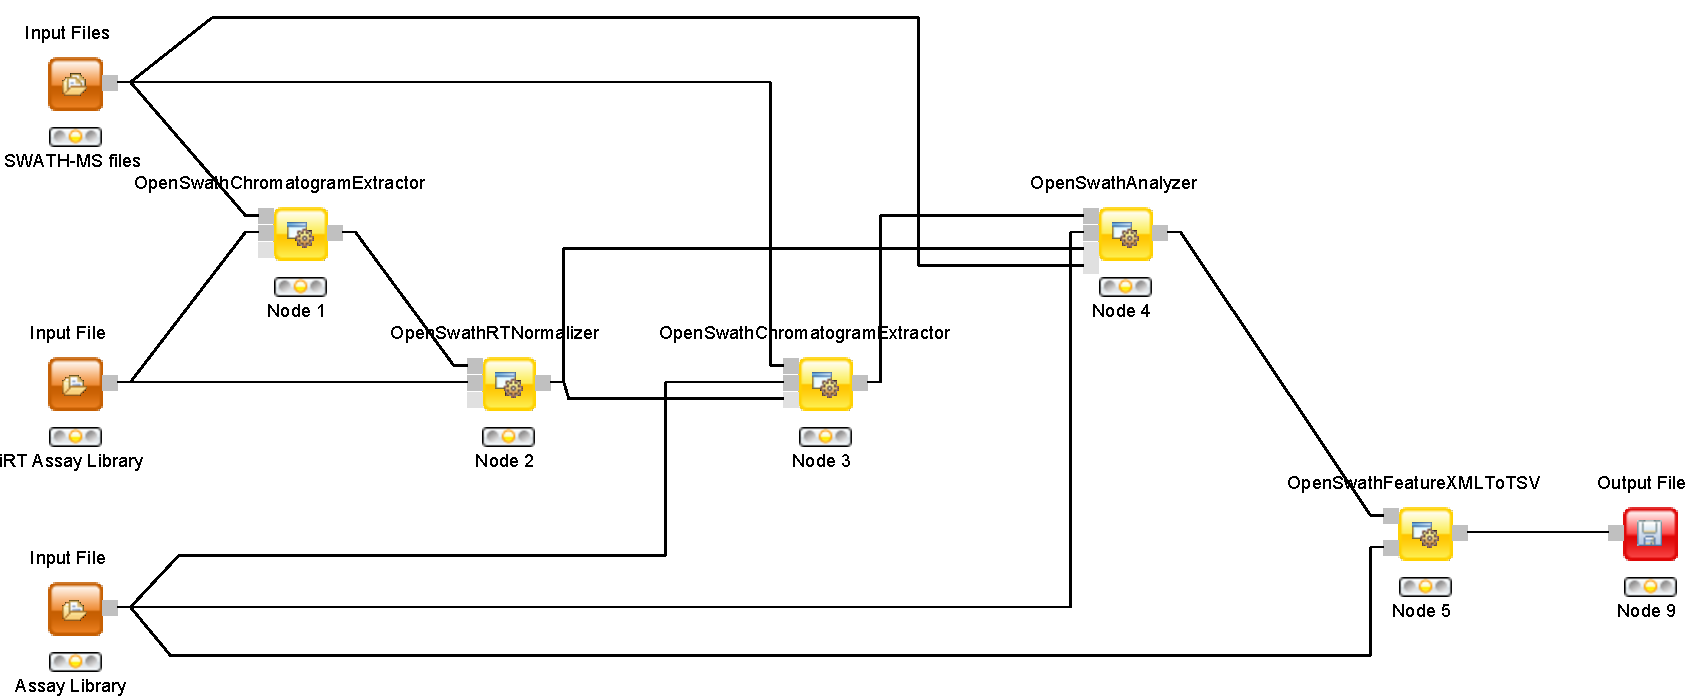
\includegraphics[width=1\textwidth]{graphics/OpenSwath}
\caption{OpenSWATH KNIME Workflow.}
\label{fig:toppas}
\end{figure*}

\subsection{From the example dataset to real-life applications}
The sample dataset used in this tutorial is part of the larger SWATH MS Gold Standard (SGS) dataset which is described in the publication of Roest et al.~\cite{Rost2014fd}.
It contains one of 90 SWATH-MS runs with significant data reduction (peak picking of the raw, profile data) to make file transfer and working with it easier. Usually SWATH-MS datasets are huge with several gigabyte per run. Especially when complex samples in combination with large assay libraries are analyzed, the TOPP tool based workflow requires a lot of computational resources. For this reason, an integrated tool (\OPENMSTOOL{OpenSwathWorkflow}) has been developed, combining all the steps shown in the KNIME-Workflow into a single executable. It is shipped with OpenMS 2.0.0. Instructions on how to use this tool can be found on \url{http://www.openswath.org}.

